% This is the Duke University Statistical Science LaTeX thesis template.
% It has been adapted from the Reed College LaTeX thesis template. The
% adaptation was done by Mine Cetinkaya-Rundel (MCR). Some of the comments
% that are specific to Reed College have been removed.
%
% Most of the work on the original Reed College document class and template
% was done by Sam Noble (SN). Later comments etc. by Ben Salzberg (BTS).
% Additional restructuring and APA support by Jess Youngberg (JY).
%
% See https://www.reed.edu/cis/help/latex/ for help. There are a
% great bunch of help pages there, with notes on
% getting started, bibtex, etc. Go there and read it if you're not
% already familiar with LaTeX.
%
% Any line that starts with a percent symbol is a comment.
% They won't show up in the document, and are useful for notes
% to yourself and explaining commands.
% Commenting also removes a line from the document;
% very handy for troubleshooting problems. -BTS

%%
%% Preamble
%%
% \documentclass{<something>} must begin each LaTeX document
\documentclass[12pt,twoside]{dukestatscithesis}
% Packages are extensions to the basic LaTeX functions. Whatever you
% want to typeset, there is probably a package out there for it.
% Chemistry (chemtex), screenplays, you name it.
% Check out CTAN to see: http://www.ctan.org/
%%
\usepackage{graphicx,latexsym}
\usepackage{amsmath}
\usepackage{amssymb,amsthm}
\usepackage{longtable,booktabs,setspace}
\usepackage{chemarr} %% Useful for one reaction arrow, useless if you're not a chem major
\usepackage[hyphens]{url}
% Added by CII
\usepackage{hyperref}
\usepackage{lmodern}
\usepackage{float}
\floatplacement{figure}{H}
% End of CII addition
\usepackage{rotating}

% Next line commented out by CII
%%% \usepackage{natbib}
% Comment out the natbib line above and uncomment the following two lines to use the new
% biblatex-chicago style, for Chicago A. Also make some changes at the end where the
% bibliography is included.
%\usepackage{biblatex-chicago}
%\bibliography{thesis}


% Added by CII (Thanks, Hadley!)
% Use ref for internal links
\renewcommand{\hyperref}[2][???]{\autoref{#1}}
\def\chapterautorefname{Chapter}
\def\sectionautorefname{Section}
\def\subsectionautorefname{Subsection}
% End of CII addition

% Added by CII
\usepackage{caption}
\captionsetup{width=5in}
% End of CII addition

% \usepackage{times} % other fonts are available like times, bookman, charter, palatino


% To pass between YAML and LaTeX the dollar signs are added by CII
\title{My Final College Paper}
\author{Nathaniel Brown}
% The month and year that you submit your FINAL draft TO THE LIBRARY (May or December)
\date{May 20xx}
\advisor{Advisor F. Name}
\institution{Duke University}
\degree{Bachelor of Science in Statistical Science}
\committeememberone{Committeemember O. Name}
\committeemembertwo{Committeemember T. Name}
\dus{Dus X. Name}
%If you have two advisors for some reason, you can use the following
% Uncommented out by CII
% End of CII addition

%%% Remember to use the correct department!
\department{Department of Statistical Science}

% Added by CII
%%% Copied from knitr
%% maxwidth is the original width if it's less than linewidth
%% otherwise use linewidth (to make sure the graphics do not exceed the margin)
\makeatletter
\def\maxwidth{ %
  \ifdim\Gin@nat@width>\linewidth
    \linewidth
  \else
    \Gin@nat@width
  \fi
}
\makeatother

\renewcommand{\contentsname}{Table of Contents}
% End of CII addition

\setlength{\parskip}{0pt}

% Added by CII

\providecommand{\tightlist}{%
  \setlength{\itemsep}{0pt}\setlength{\parskip}{0pt}}

\Acknowledgements{
I want to thank a few people.
}

\Dedication{
You can have a dedication here if you wish.
}

\Preface{
This is an example of a thesis setup to use the reed thesis document
class (for LaTeX) and the R bookdown package, in general.
}

\Abstract{
\chapter{Abstract}\label{abstract}

The proposed study is an investigation of Bayesian statistical models
and analyses for problems arising in shooting a basketball. The data
comes from the Duke Men's Basketball team's player-tracking data from
the SportVU cameras of STATS, LLC. Goals will be to explore, develop and
apply Bayesian models to existing and new data on shooting outcomes, to
understand and evaluate questions of inherent random variation, changes
over time in shooting performance, and issues related to the ``Hot
Hand'' concept in sports.

\par

The models we use to investigate this data are a Generalized Linear
Model, a Dynamic Generalized Linear Model, and a Bayesian Hierarchichal
Model.

\par

Our results so far show that the best-fitting model is a Dynamic
Generalized Linear Model; this suggests that the predictive features of
a shooting model may be time-dependent.
}

% End of CII addition
%%
%% End Preamble
%%
%

\usepackage{amsthm}
\newtheorem{theorem}{Theorem}[chapter]
\newtheorem{lemma}{Lemma}[chapter]
\theoremstyle{definition}
\newtheorem{definition}{Definition}[chapter]
\newtheorem{corollary}{Corollary}[chapter]
\newtheorem{proposition}{Proposition}[chapter]
\theoremstyle{definition}
\newtheorem{example}{Example}[chapter]
\theoremstyle{definition}
\newtheorem{exercise}{Exercise}[chapter]
\theoremstyle{remark}
\newtheorem*{remark}{Remark}
\newtheorem*{solution}{Solution}
\begin{document}

% Everything below added by CII
  \maketitle

\frontmatter % this stuff will be roman-numbered
\pagestyle{empty} % this removes page numbers from the frontmatter
  \begin{acknowledgements}
    I want to thank a few people.
  \end{acknowledgements}
  \begin{preface}
    This is an example of a thesis setup to use the reed thesis document
    class (for LaTeX) and the R bookdown package, in general.
  \end{preface}
  \hypersetup{linkcolor=black}
  \setcounter{tocdepth}{2}
  \tableofcontents

  \listoftables

  \listoffigures
  \begin{abstract}
    \chapter{Abstract}\label{abstract}
    
    The proposed study is an investigation of Bayesian statistical models
    and analyses for problems arising in shooting a basketball. The data
    comes from the Duke Men's Basketball team's player-tracking data from
    the SportVU cameras of STATS, LLC. Goals will be to explore, develop and
    apply Bayesian models to existing and new data on shooting outcomes, to
    understand and evaluate questions of inherent random variation, changes
    over time in shooting performance, and issues related to the ``Hot
    Hand'' concept in sports.
    
    \par
    
    The models we use to investigate this data are a Generalized Linear
    Model, a Dynamic Generalized Linear Model, and a Bayesian Hierarchichal
    Model.
    
    \par
    
    Our results so far show that the best-fitting model is a Dynamic
    Generalized Linear Model; this suggests that the predictive features of
    a shooting model may be time-dependent.
  \end{abstract}
  \begin{dedication}
    You can have a dedication here if you wish.
  \end{dedication}
\mainmatter % here the regular arabic numbering starts
\pagestyle{fancyplain} % turns page numbering back on

\chapter*{Introduction}\label{introduction}
\addcontentsline{toc}{chapter}{Introduction}

Welcome to the \emph{R Markdown} thesis template. This template is based
on (and in many places copied directly from) the Reed College LaTeX
template, but hopefully it will provide a nicer interface for those that
have never used TeX or LaTeX before. Using \emph{R Markdown} will also
allow you to easily keep track of your analyses in \textbf{R} chunks of
code, with the resulting plots and output included as well. The hope is
this \emph{R Markdown} template gets you in the habit of doing
reproducible research, which benefits you long-term as a researcher, but
also will greatly help anyone that is trying to reproduce or build onto
your results down the road.

Hopefully, you won't have much of a learning period to go through and
you will reap the benefits of a nicely formatted thesis. The use of
LaTeX in combination with \emph{Markdown} is more consistent than the
output of a word processor, much less prone to corruption or crashing,
and the resulting file is smaller than a Word file. While you may have
never had problems using Word in the past, your thesis is likely going
to be about twice as large and complex as anything you've written
before, taxing Word's capabilities. After working with \emph{Markdown}
and \textbf{R} together for a few weeks, we are confident this will be
your reporting style of choice going forward.

\textbf{Why use it?}

\emph{R Markdown} creates a simple and straightforward way to interface
with the beauty of LaTeX. Packages have been written in \textbf{R} to
work directly with LaTeX to produce nicely formatting tables and
paragraphs. In addition to creating a user friendly interface to LaTeX,
\emph{R Markdown} also allows you to read in your data, to analyze it
and to visualize it using \textbf{R} functions, and also to provide the
documentation and commentary on the results of your project. Further, it
allows for \textbf{R} results to be passed inline to the commentary of
your results. You'll see more on this later.

Having your code and commentary all together in one place has a plethora
of benefits!

\textbf{Who should use it?}

Anyone who needs to use data analysis, math, tables, a lot of figures,
complex cross-references, or who just cares about the final appearance
of their document should use \emph{R Markdown}. Of particular use should
be anyone in the sciences, but the user-friendly nature of
\emph{Markdown} and its ability to keep track of and easily include
figures, automatically generate a table of contents, index, references,
table of figures, etc. should make it of great benefit to nearly anyone
writing a thesis project.

\chapter{Abstract}\label{abstract}

The proposed study is an investigation of Bayesian statistical models
and analyses for problems arising in shooting a basketball. The data
comes from the Duke Men's Basketball team's player-tracking data from
the SportVU cameras of STATS, LLC. Goals will be to explore, develop and
apply Bayesian models to existing and new data on shooting outcomes, to
understand and evaluate questions of inherent random variation, changes
over time in shooting performance, and issues related to the ``Hot
Hand'' concept in sports.

\par

The models we use to investigate this data are a Generalized Linear
Model, a Dynamic Generalized Linear Model, and a Bayesian Hierarchichal
Model.

\par

Our results so far show that the best-fitting model is a Dynamic
Generalized Linear Model; this suggests that the predictive features of
a shooting model may be time-dependent.

\chapter{Literature Review}\label{litreview}

\subsection{how do I get the full citations to show up and not just last
name and
year?}\label{how-do-i-get-the-full-citations-to-show-up-and-not-just-last-name-and-year}

Gilovich, Vallone, \& Tversky (1985)

In this research paper from \emph{Cognitive Psychology}, Thomas
Gilovich, Robert Vallone, and Amos Tversky investigate peoples' belief
in the Hot Hand in Basketball. The Hot Hand is the concept that the
probability of a success increases for trials that follow a success in a
binary sequence; in basketball, these binary events are shot attempts.
The methods in this paper include an analysis of shot attempts from the
Philadelphia 76ers of the National Basketball Association (NBA) in the
1981 season, analysis of free-throw attempts from the Boston Celtics in
the 1981 and 1982 seasons, and a controlled shooting drill using male
and female varsity basketball players at Cornell University. Statistical
techniques they used to attempt to detect streakiness in the data
included Walf-Wolfowitz run tests, autocorrelation tests on consecutive
shot attempts, goodness-of-fit tests for the distribution of succesess,
and paired t-tests comparing the mean of makes following a make to that
of makes following a miss. In addition to this analysis of shooting,
this research also contained a survey of basketball fans, that gauged
how much people believed success probabilities changed given a success
or a failure. The statistical tests did not detect significant evidence
supporting the Hot Hand in basketball. The lack of statistical power in
Gilovich, Vallone, and Tversky's frequentist tests motivates the use of
Bayesian models in this thesis. Strengths of this paper include the fact
that it was one of the first research papers to analyze streakiness in
basketball data, and many future papers build off of it. Some weaknesses
in this paper are the assumptions it makes in its analysis, such as all
shots being independent of each other, and not accounting for shot
location. Albert \& Williamson (1999)

In this paper, Jim Albert attempts to improve upon the low-powered tests
of Gilovich, Vallone, and Tverky's 1985 paper on the Hot Hand. Albert
formally defines ``streakiness'' as the presence of nonstationarity
(nonconstant probability between trials) or autocorrelation (sequential
dependency). Albert uses Gibbs sampling to approximate posterior
densities and to simulate data, then fits two types of models on binary
data from baseball and basketball to try to characterize streakiness. He
fits an overdispersion model to detect nonstationarity, and a markov
switching model to detect sequential dependencies. While he did not
uncover strong evidence for the hot hand, one of his takeaways was that
overdispersion decreases as time goes on in basketball free throw
shooting data. A weakness of this paper is that Albert does not show the
results of both the Markov model and the overdispersion model on the
same data. We use Albert's formal definitions of streakiness as well as
his motivation for Bayesian models over frequentist tests.

Bar-Eli, Avugos, \& Raab (2006)

This paper is a review of previous hot hand research. It reviews several
papers investigating the concept of the ``hot hand'' in several sports
such as basketball, baseball, volleyball, and horeshoe, and other fields
such as cognitive science and economics. Bar-Eli, Avugos, and Raab
evaluate the datasets, the tests and statistics used, and the
conclusions of each study. Overall, the authors summarize 13 papers that
oppose the hot hand phenomenon, and 11 that support it; they also
acknowledge that the scientific evidence for the hot hand is weaker than
the evidence against it, and it is typically more controversial. Instead
of just looking to answer whether the hot hand exists, Bar-Eli, Avugos,
and Raab also examine how people define a ``hot hand'', and the
psychological factors behind the belief in it, such as the gambling and
game strategy. The strengths of this paper are that it evaluates the
strengths and weaknesses of many competing claims, and concisely
summarizes the information into a table. A weakness is that they do not
make any claim of their own. This paper is useful in this thesis because
it describes several data analysis techniques to detect streaks in a
binary sequence.

Ryan Wetzels (2016)

In this research paper, Wetzels conducts a simulation study to
investigate the Hot Hand Phenomenon. His analysis consists of
calculating Bayes Factors to compare evidence between a Hidden Markov
Model with two states and a binomial model with one state. He applies
this method to data from basketball foul shots and from visual
discernment tests. In the basketball data, he found that Shaquille
O'Neal's free-throws show evidence for a two-state Markov model, while
Kobe Bryant's show more evidence for a one-state binomial model. In the
data from the visual discernment tests, he found no strong evidence
supporting one model over the other. A strength of this paper is
Wetzel's formal comparison of a Bayesian Markov model to a binomial
model. A weakness is that the Bayes Factors only compare evidence
between the two models; it does not mean that either model is ``good''.
We use this paper for the specification of the Hidden Markov Model.

Albert (1993)

In this paper, Albert uses a Markov switching model to analyze
streakiness in baseball pitching data. He concludes that a few players
exhibit streakiness, but not enough to reject the null hypothesis. An
exploratory technique that we take from this paper is to examine the
peaks and valleys in a moving average plot to observe streakiness. A
strength of this paper is that Albert controls for situational variables
such as home field advantage, the handedness of the pitcher, and the
runners on the bases.

Albert (2013)

In this paper, Albert analyzes streakiness in baseball hitting data. His
analysis techniques include using Bayes Factors to compare models of the
form \(f(y_j|p_j) = p_j(1-p_j)^{y_j}, y_j = 0,1,2,...\); a consistent
model with a constant \(p_j\), and a streaky model with a varying
\(p_j\) from a beta distribution. A useful insight that we apply to this
paper is the concept that the existence of streakiness depends on the
definition of ``success'' in binary outcome data. He found substantially
more evidence for streakiness for when a success was coded as ``not a
strikeout'' instead of a ``hit''. Likewise, in this paper we
\emph{blank}.

West, Harrison, \& Migon (1985)

This textbook provides theory, applications, and examples of time series
models such Dynamic Generalized Linear Models (DGLMs). More
specifically, section 14.4 provides an example of a DGLM for a binomial
response variable, which we apply in chapter \emph{blank} of this
research paper.

\chapter{Data}\label{data}

The data for this analysis comes from SportVU, a player-tracking system
from STATS, LLC. that provides precise coordinates for all ten players
and the ball at a rate of 25 times per second. The Duke University Men's
Basketball team permitted the use of their SportVU data from the 2014 to
2017 basketball seasons for this project. However, since the ability to
record this data depends on specialized tracking cameras, Duke does not
have this data for every game they play---only home games, and a few
road games in arenas that had the techology installed. Therefore, there
is a substantial amount of missing data between games.

For our analysis, we use the following files for each game:
\begin{itemize}
\item
  Final Sequence Play-by-Play Optical:

  This dataset comes in an a semi-structured Extensible Markup Language
  (XML) file, where there is a unique element for each ``event'' (an
  event is a basketball action such as a dribble, pass, shot, foul,
  etc.). Each event element has attributes describing the type of event,
  the time of the event, and the player who completed the action. We use
  these files to uncover when a shot is attempted in a game, who
  attempted the shot, and the result of the shot attempt.
\item
  Box Score Optical:

  We use this dataset to match the names and ids of players who were in
  the game. This is also an XML file, with elements corresponding to
  individual players. These elements contain attributes describing
  information about the player (e.g.~team name, jersey number) and
  various statistics for the game (e.g.~points, assists, distance run).
\item
  Final Sequence Optical:

  These XML files contain the locations of all ten players and the ball
  during precise time intervals within the game. Each timeunit has a
  unique element, and these elements have attributes describing the
  locations. We merge this with the Final Sequence Play-by-Play Optical
  data on the time attribute to obtain the shooter's location at the
  moment of a shot attempt.

  \textless{}!--
\item
  Final Box Optical:
\end{itemize}
These file contain semi-structured data --\textgreater{}

\chapter{Procedure}\label{proc}

Using the time-stamped sequence of shot locations and binary outcomes,
we fit generalized linear models, dynamic generalized linear models, or
DGLMs (West, Migon, and Harrison, 1985) (West and Harrison, 1997), and
hierarchichal models. DGLMs allow for time-varying effects on shot
attempt frequency and shot success rate within a game and between games.
The formal Bayesian analysis allows us to produce full quantified
inferences on these patterns over time, with probabilistic summaries of
the within-game and between-game outcomes. For each provided game, we
will analyze player shooting tendencies and outcomes, which provides
understanding of inherent variability (or ``randomness'') for the
players, and formal assessments of differences in patterns game-to-game.

We are also considering a two-state Hidden Markov Switching Model that
parallels and extends these models; the two potential states for each
shot attempt are a ``high'' probability or a ``low'' probability of
making the next shot, given the features of the current and previous
possessions.

\chapter{Exploratory Data Analysis}\label{EDA}

\subsubsection{Exploratory Data
Analysis}\label{exploratory-data-analysis}

The following exploratory plots examine how consistent the probability
of a made shot is, using a loess smooth curve on the binary outcomes. We
present these smoothed plots for four high-usage basketball players at
Duke University, and we leave the others in the Appendix. Each plot
represents a single player's ordered shooting outcomes for a single
season. These plots do not account for the amount of time in between
shots, but simply shot order and outcome.
\begin{Shaded}
\begin{Highlighting}[]
\NormalTok{datafolder <-}\StringTok{ "C:/Users/Nathaniel Brown/Documents/important things/DMBBall Data/"}
\NormalTok{githubfolder <-}\StringTok{ "C:/Users/Nathaniel Brown/Documents/GitHub/thesis-sp18-brown-hothand/"}
\KeywordTok{source}\NormalTok{(}\KeywordTok{paste0}\NormalTok{(githubfolder,}\StringTok{"sportvu_fxns.R"}\NormalTok{))}
\end{Highlighting}
\end{Shaded}
\begin{verbatim}
Warning: package 'xml2' was built under R version 3.3.3
\end{verbatim}
\begin{Shaded}
\begin{Highlighting}[]
\NormalTok{plotshottime <-}\StringTok{ }\NormalTok{function(playerid, season)\{}
  \NormalTok{allgameshots_sub <-}\StringTok{ }\NormalTok{allgameshots[allgameshots$globalplayerid==playerid &}\StringTok{ }\NormalTok{allgameshots$season==season,]}
  \NormalTok{if(}\KeywordTok{nrow}\NormalTok{(allgameshots_sub) <}\StringTok{ }\DecValTok{10}\NormalTok{)\{}
    \KeywordTok{plot}\NormalTok{(}\DecValTok{0}\NormalTok{,}\DecValTok{0}\NormalTok{,}\DataTypeTok{type=}\StringTok{"n"}\NormalTok{, }\DataTypeTok{yaxt=}\StringTok{"n"}\NormalTok{,}\DataTypeTok{xaxt=}\StringTok{"n"}\NormalTok{, }\DataTypeTok{ylab=}\StringTok{""}\NormalTok{,}\DataTypeTok{xlab=}\StringTok{""}\NormalTok{)}
    \KeywordTok{text}\NormalTok{(}\DecValTok{0}\NormalTok{,}\DecValTok{0}\NormalTok{,}\DataTypeTok{label=}\StringTok{"Not Enough Data"}\NormalTok{, }\DataTypeTok{cex=}\DecValTok{2}\NormalTok{)}
  \NormalTok{\}else\{}
    \NormalTok{Y <-}\StringTok{ }\NormalTok{allgameshots_sub$result }\CommentTok{#zoo::rollmean((allgameshots_sub$result), 4)}
    \NormalTok{X <-}\StringTok{ }\DecValTok{1}\NormalTok{:}\KeywordTok{length}\NormalTok{(Y)}
    \KeywordTok{scatter.smooth}\NormalTok{(X,Y,}\DataTypeTok{span=}\DecValTok{20}\NormalTok{/}\KeywordTok{length}\NormalTok{(Y), }\DataTypeTok{main =} \KeywordTok{paste0}\NormalTok{(}\StringTok{"Smoothed Shooting Outcomes"}\NormalTok{),}
                   \DataTypeTok{yaxt=}\StringTok{"n"}\NormalTok{,}\DataTypeTok{ylab=}\StringTok{"Result"}\NormalTok{,}\DataTypeTok{xlab=}\StringTok{"Order"}\NormalTok{)}
    \KeywordTok{axis}\NormalTok{(}\DataTypeTok{side=}\DecValTok{2}\NormalTok{,}\DataTypeTok{at=}\KeywordTok{c}\NormalTok{(}\DecValTok{0}\NormalTok{,}\DecValTok{1}\NormalTok{),}\DataTypeTok{labels=}\KeywordTok{c}\NormalTok{(}\StringTok{"Miss"}\NormalTok{,}\StringTok{"Make"}\NormalTok{))}
  \NormalTok{\}}
\NormalTok{\}}

\NormalTok{maxseason <-}\StringTok{ }\NormalTok{allgameshots %>%}\StringTok{ }\KeywordTok{group_by}\NormalTok{(globalplayerid, season) %>%}\StringTok{ }\KeywordTok{summarize}\NormalTok{(}\DataTypeTok{num=}\KeywordTok{n}\NormalTok{()) %>%}\StringTok{ }\KeywordTok{group_by}\NormalTok{(globalplayerid) %>%}\StringTok{ }\KeywordTok{mutate}\NormalTok{(}\DataTypeTok{m=}\KeywordTok{max}\NormalTok{(num)) %>%}\StringTok{ }\KeywordTok{filter}\NormalTok{(num==m) %>%}\StringTok{ }\KeywordTok{as.data.frame}\NormalTok{()}
\end{Highlighting}
\end{Shaded}
\begin{verbatim}
Warning: package 'bindrcpp' was built under R version 3.3.3
\end{verbatim}
\begin{Shaded}
\begin{Highlighting}[]
\NormalTok{for(i in }\DecValTok{1}\NormalTok{:}\KeywordTok{nrow}\NormalTok{(playerseasons))\{}
  \NormalTok{r <-}\StringTok{ }\NormalTok{playerseasons[i,]}
  \KeywordTok{plotshottime}\NormalTok{(r[[}\DecValTok{1}\NormalTok{]],r[[}\DecValTok{2}\NormalTok{]])}
\NormalTok{\}}
\end{Highlighting}
\end{Shaded}
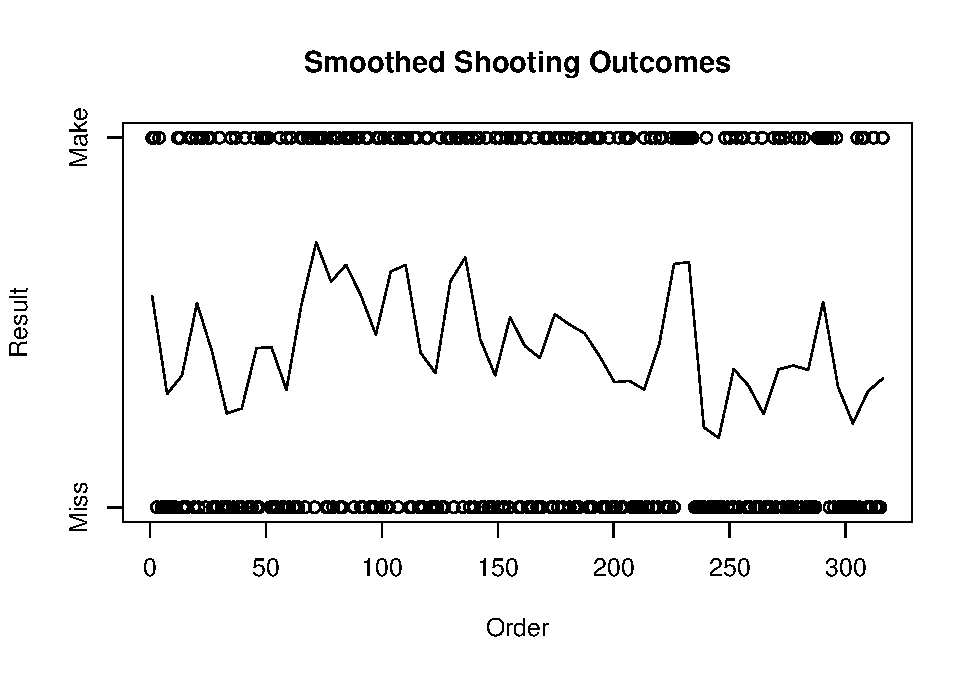
\includegraphics{thesis_files/figure-latex/plots-1.pdf}
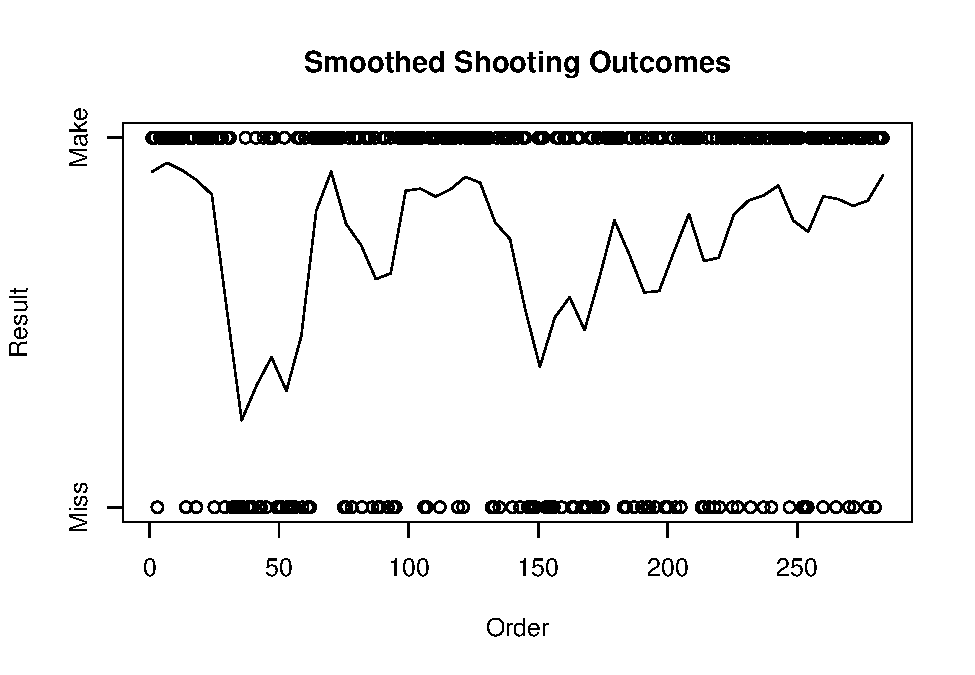
\includegraphics{thesis_files/figure-latex/plots-2.pdf}
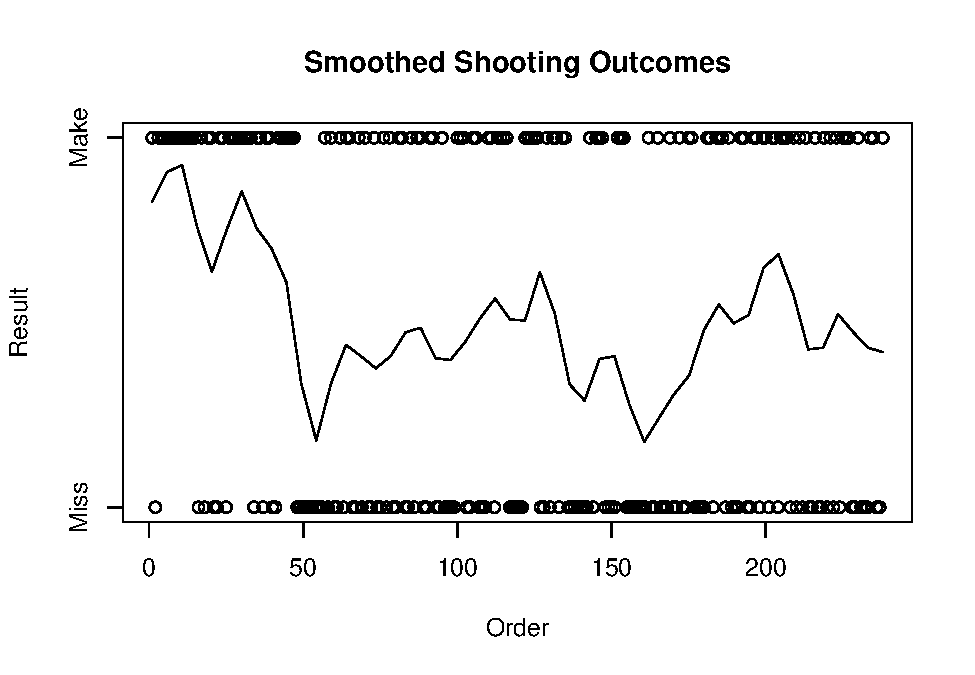
\includegraphics{thesis_files/figure-latex/plots-3.pdf}
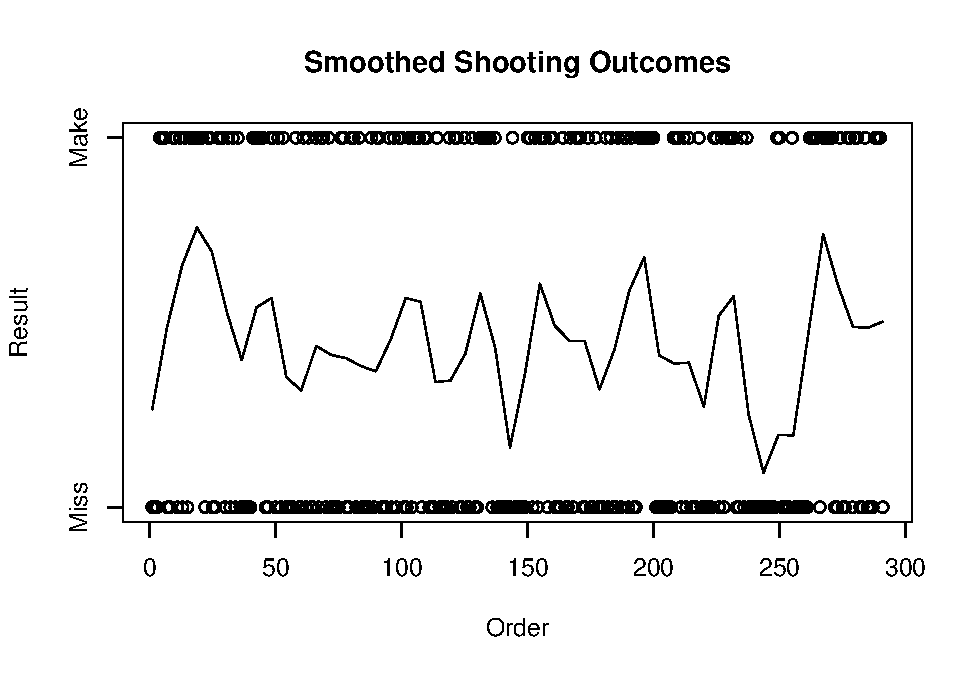
\includegraphics{thesis_files/figure-latex/plots-4.pdf}

We can see that the plots vary in the consistency of their made shots,
since they all contain spikes and trends. For example, the third plot
initially has a very high success rate, which quickly falls to the
middle after about thirty shot attempts, and the second plot has a
noticeable upward trend in shot success beginning around shot number one
hundred fifty.

We investigate the shooting outcome using Bayesian models, and show the
results in the next section.
\begin{verbatim}
NULL
NULL
\end{verbatim}
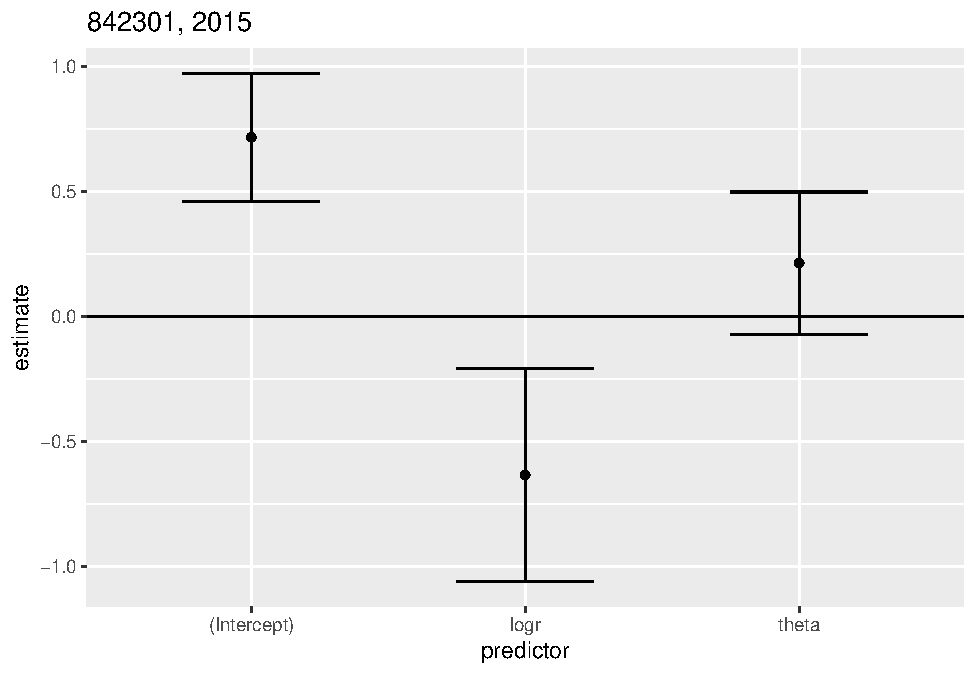
\includegraphics{thesis_files/figure-latex/unnamed-chunk-1-2.pdf}
\begin{verbatim}
NULL
NULL
\end{verbatim}
--\textgreater{}

\chapter{Models}\label{model}

For our models, we consider the shot location and the shooter identity
as factors that can affect a shot outcome. For each of the following
models, shot location is parametrized in polar coordinates, or \(r\) and
\(\theta\).

\subsubsection{Generalized Linear Model}\label{generalized-linear-model}

The results of the credible intervals are reported for the same four
players, in the same order.
\begin{Shaded}
\begin{Highlighting}[]
\CommentTok{# playerid <- id2}
\CommentTok{# seasons <- c(2014,2015,2016,2017)}

\NormalTok{priormod <-}\StringTok{ }\KeywordTok{glm}\NormalTok{(result ~}\StringTok{ }\KeywordTok{log}\NormalTok{(r) +}\StringTok{ }\NormalTok{theta, }\DataTypeTok{data=}\NormalTok{allgameshots %>%}\StringTok{ }\KeywordTok{filter}\NormalTok{(}\KeywordTok{as.integer}\NormalTok{(}\KeywordTok{as.factor}\NormalTok{(gameid)) <}\StringTok{ }\DecValTok{5}\NormalTok{), }\DataTypeTok{family=}\StringTok{"binomial"}\NormalTok{)}
\NormalTok{mu0r <-}\StringTok{ }\KeywordTok{summary}\NormalTok{(priormod)[[}\StringTok{"coefficients"}\NormalTok{]][}\StringTok{"log(r)"}\NormalTok{,}\StringTok{"Estimate"}\NormalTok{]}
\NormalTok{mu0theta <-}\StringTok{ }\KeywordTok{summary}\NormalTok{(priormod)[[}\StringTok{"coefficients"}\NormalTok{]][}\StringTok{"log(r)"}\NormalTok{,}\StringTok{"Std. Error"}\NormalTok{]}
\NormalTok{tau0r <-}\StringTok{ }\KeywordTok{summary}\NormalTok{(priormod)[[}\StringTok{"coefficients"}\NormalTok{]][}\StringTok{"theta"}\NormalTok{,}\StringTok{"Std. Error"}\NormalTok{]^}\DecValTok{2}
\NormalTok{tau0theta <-}\StringTok{ }\KeywordTok{summary}\NormalTok{(priormod)[[}\StringTok{"coefficients"}\NormalTok{]][}\StringTok{"theta"}\NormalTok{,}\StringTok{"Std. Error"}\NormalTok{]^}\DecValTok{2}


\NormalTok{fit_glm <-}\StringTok{ }\NormalTok{function(playerids, }\DataTypeTok{seasons =} \DecValTok{2014}\NormalTok{:}\DecValTok{2017}\NormalTok{)\{}
  
  \NormalTok{model.glm <-}\StringTok{ }\NormalTok{function()\{}
  
    \CommentTok{# N observations}
    \NormalTok{for(i in }\DecValTok{1}\NormalTok{:N)\{}
      \NormalTok{result[i] ~}\StringTok{ }\KeywordTok{dbern}\NormalTok{(prob[i])}
      \KeywordTok{logit}\NormalTok{(prob[i]) <-}\StringTok{ }\NormalTok{beta_int*int[i] +}\StringTok{ }\NormalTok{beta_r*logr[i] +}\StringTok{ }\NormalTok{beta_theta*theta[i]}
    \NormalTok{\}}

    \CommentTok{# Priors}
    \NormalTok{beta_int   ~}\StringTok{ }\KeywordTok{dnorm}\NormalTok{(}\DecValTok{0}\NormalTok{, }\FloatTok{0.1}\NormalTok{)}
    \NormalTok{beta_r     ~}\StringTok{ }\KeywordTok{dnorm}\NormalTok{(mu0r, }\FloatTok{0.01}\NormalTok{) }\CommentTok{#would not expect a lot of variation in distance parameter between players. Everyone should get worse as distance increases.}
    \NormalTok{beta_theta ~}\StringTok{ }\KeywordTok{dnorm}\NormalTok{(mu0theta, }\FloatTok{0.1}\NormalTok{)}

  \NormalTok{\}}

  \NormalTok{allgameshots_sub <-}\StringTok{ }\NormalTok{allgameshots %>%}\StringTok{ }\KeywordTok{filter}\NormalTok{(globalplayerid %in%}\StringTok{ }\NormalTok{playerids &}
\StringTok{                                            }\NormalTok{season %in%}\StringTok{ }\NormalTok{seasons)}

  \NormalTok{datlist.glm <-}\StringTok{  }\KeywordTok{list}\NormalTok{(}
                    \DataTypeTok{logr =} \KeywordTok{log}\NormalTok{(allgameshots_sub$r), }
                    \DataTypeTok{theta =} \NormalTok{allgameshots_sub$theta, }
                    \DataTypeTok{result =} \NormalTok{allgameshots_sub$result, }
                    \DataTypeTok{N =} \KeywordTok{nrow}\NormalTok{(allgameshots_sub), }
                    \DataTypeTok{int =} \KeywordTok{rep}\NormalTok{(}\DecValTok{1}\NormalTok{, }\KeywordTok{nrow}\NormalTok{(allgameshots_sub)), }
                    \DataTypeTok{mu0r =} \NormalTok{mu0r,}
                    \DataTypeTok{mu0theta =} \NormalTok{mu0theta}
                \NormalTok{)}
  \NormalTok{params.glm <-}\StringTok{ }\KeywordTok{c}\NormalTok{(}\StringTok{"beta_int"}\NormalTok{,}\StringTok{"beta_r"}\NormalTok{, }\StringTok{"beta_theta"}\NormalTok{)}


  \NormalTok{sim <-}\StringTok{ }\KeywordTok{jags}\NormalTok{(}\DataTypeTok{data =} \NormalTok{datlist.glm, }
              \DataTypeTok{n.iter =} \DecValTok{10000}\NormalTok{, }\DataTypeTok{n.chains =} \DecValTok{1}\NormalTok{, }\DataTypeTok{n.burnin =} \DecValTok{500}\NormalTok{,}
              \CommentTok{#inits=list(list(p = rep(0.5, nrow(P0)))),}
              \DataTypeTok{parameters.to.save =} \NormalTok{params.glm,}
              \DataTypeTok{model.file=}\NormalTok{model.glm}
  \NormalTok{)}
  \NormalTok{sim.mcmc <-}\StringTok{ }\KeywordTok{as.data.frame}\NormalTok{(}\KeywordTok{as.mcmc}\NormalTok{(sim)[[}\DecValTok{1}\NormalTok{]])}
  \KeywordTok{return}\NormalTok{(sim.mcmc)}
\NormalTok{\}}



\NormalTok{plot_params <-}\StringTok{ }\NormalTok{function(}\DataTypeTok{sim.mcmc =} \OtherTok{NA}\NormalTok{)\{}
  
    \NormalTok{coefs <-}\StringTok{ }\NormalTok{sim.mcmc[,}\KeywordTok{c}\NormalTok{(}\StringTok{"beta_int"}\NormalTok{,}\StringTok{"beta_r"}\NormalTok{,}\StringTok{"beta_theta"}\NormalTok{)] %>%}\StringTok{ }\KeywordTok{apply}\NormalTok{(}\DecValTok{2}\NormalTok{, quantile, }\KeywordTok{c}\NormalTok{(}\FloatTok{0.025}\NormalTok{,}\FloatTok{0.5}\NormalTok{,}\FloatTok{0.975}\NormalTok{)) %>%}\StringTok{ }\KeywordTok{t}\NormalTok{() %>%}\StringTok{ }\KeywordTok{as.data.frame}\NormalTok{()}
    
    \KeywordTok{colnames}\NormalTok{(coefs) <-}\StringTok{ }\KeywordTok{c}\NormalTok{(}\StringTok{"lo"}\NormalTok{, }\StringTok{"mid"}\NormalTok{, }\StringTok{"hi"}\NormalTok{)}
  
    \KeywordTok{ggplot}\NormalTok{(}\DataTypeTok{data =} \NormalTok{coefs, }\KeywordTok{aes}\NormalTok{(}\DataTypeTok{x=}\KeywordTok{c}\NormalTok{(}\StringTok{"intercept"}\NormalTok{,}\StringTok{"distance"}\NormalTok{,}\StringTok{"angle"}\NormalTok{),}\DataTypeTok{y=}\NormalTok{mid)) +}\StringTok{ }
\StringTok{      }\KeywordTok{geom_point}\NormalTok{() +}\StringTok{ }
\StringTok{      }\KeywordTok{geom_errorbar}\NormalTok{(}\KeywordTok{aes}\NormalTok{(}\DataTypeTok{ymin=}\NormalTok{lo, }\DataTypeTok{ymax=}\NormalTok{hi), }\DataTypeTok{width=}\FloatTok{0.5}\NormalTok{) +}\StringTok{ }
\StringTok{      }\KeywordTok{geom_abline}\NormalTok{(}\DataTypeTok{intercept=}\DecValTok{0}\NormalTok{, }\DataTypeTok{slope=}\DecValTok{0}\NormalTok{, }\DataTypeTok{linetype=}\DecValTok{2}\NormalTok{) +}\StringTok{ }
\StringTok{      }\KeywordTok{labs}\NormalTok{(}\DataTypeTok{title=}\StringTok{"GLM Posterior Parameters (95% error)"}\NormalTok{,}\DataTypeTok{x=}\StringTok{"predictor"}\NormalTok{, }\DataTypeTok{y=}\StringTok{"estimate"}\NormalTok{) +}\StringTok{ }
\StringTok{      }\KeywordTok{theme_bw}\NormalTok{()}
\NormalTok{\}}

\NormalTok{playerseasons}
\NormalTok{glm1 <-}\StringTok{ }\KeywordTok{fit_glm}\NormalTok{(playerseasons[}\DecValTok{1}\NormalTok{,}\DecValTok{1}\NormalTok{], playerseasons[}\DecValTok{1}\NormalTok{,}\DecValTok{2}\NormalTok{])}
\NormalTok{glm2 <-}\StringTok{ }\KeywordTok{fit_glm}\NormalTok{(playerseasons[}\DecValTok{2}\NormalTok{,}\DecValTok{1}\NormalTok{], playerseasons[}\DecValTok{2}\NormalTok{,}\DecValTok{2}\NormalTok{])}
\NormalTok{glm3 <-}\StringTok{ }\KeywordTok{fit_glm}\NormalTok{(playerseasons[}\DecValTok{3}\NormalTok{,}\DecValTok{1}\NormalTok{], playerseasons[}\DecValTok{3}\NormalTok{,}\DecValTok{2}\NormalTok{])}
\NormalTok{glm4 <-}\StringTok{ }\KeywordTok{fit_glm}\NormalTok{(playerseasons[}\DecValTok{4}\NormalTok{,}\DecValTok{1}\NormalTok{], playerseasons[}\DecValTok{4}\NormalTok{,}\DecValTok{2}\NormalTok{])}

\KeywordTok{plot_params}\NormalTok{(glm1)}
\KeywordTok{plot_params}\NormalTok{(glm2)}
\KeywordTok{plot_params}\NormalTok{(glm3)}
\KeywordTok{plot_params}\NormalTok{(glm4)}
\end{Highlighting}
\end{Shaded}
The four plots show the GLM parameters for the four players and seasons
that we investigated in the Exploratory Data Analysis section. From
these plots we see that the effect of the angle contains zero, and it is
probably not predictive of a made shot. We also see that the 95\%
credible interval on the effect of distance is completely negative,
which follows the intuitive idea that the probability of a made shot
decreases as distance from the basket increases.

\subsubsection{Hierarchichal Model}\label{hierarchichal-model}
\begin{Shaded}
\begin{Highlighting}[]
\NormalTok{priormod <-}\StringTok{ }\KeywordTok{glm}\NormalTok{(result ~}\StringTok{ }\KeywordTok{log}\NormalTok{(r) +}\StringTok{ }\NormalTok{theta, }\DataTypeTok{data=}\NormalTok{allgameshots %>%}\StringTok{ }\KeywordTok{filter}\NormalTok{(}\KeywordTok{as.integer}\NormalTok{(}\KeywordTok{as.factor}\NormalTok{(gameid)) <}\StringTok{ }\DecValTok{5}\NormalTok{), }\DataTypeTok{family=}\StringTok{"binomial"}\NormalTok{)}
\NormalTok{mu0r <-}\StringTok{ }\KeywordTok{summary}\NormalTok{(priormod)[[}\StringTok{"coefficients"}\NormalTok{]][}\StringTok{"log(r)"}\NormalTok{,}\StringTok{"Estimate"}\NormalTok{]}
\NormalTok{mu0theta <-}\StringTok{ }\KeywordTok{summary}\NormalTok{(priormod)[[}\StringTok{"coefficients"}\NormalTok{]][}\StringTok{"log(r)"}\NormalTok{,}\StringTok{"Std. Error"}\NormalTok{]}
\NormalTok{tau0r <-}\StringTok{ }\KeywordTok{summary}\NormalTok{(priormod)[[}\StringTok{"coefficients"}\NormalTok{]][}\StringTok{"theta"}\NormalTok{,}\StringTok{"Std. Error"}\NormalTok{]^}\DecValTok{2}
\NormalTok{tau0theta <-}\StringTok{ }\KeywordTok{summary}\NormalTok{(priormod)[[}\StringTok{"coefficients"}\NormalTok{]][}\StringTok{"theta"}\NormalTok{,}\StringTok{"Std. Error"}\NormalTok{]^}\DecValTok{2}

\CommentTok{# model2 <- function()\{}
\CommentTok{#     # N observations}
\CommentTok{#     for(i in 1:N)\{}
\CommentTok{#       result[i] ~ dbern(prob[i])}
\CommentTok{#       logit(prob[i]) <- beta_int*int[i] + e_int[player[i]] + beta_r*logr[i] + e_r[player[i]] + beta_theta*theta[i] + e_theta[player[i]] # a random 'e' here or is that implied?}
\CommentTok{#     \}}
\CommentTok{#     # priors on random player effects}
\CommentTok{#     for(j in 1:M)\{}
\CommentTok{#         e_int[j] ~ dnorm(beta_int,tau)}
\CommentTok{#         e_r[j] ~ dnorm(beta_r,tau)}
\CommentTok{#         e_theta[j] ~ dnorm(beta_theta,tau)}
\CommentTok{#     \}}
\CommentTok{#     # Priors}
\CommentTok{#     beta_int   ~ dnorm(0.0,0.1)}
\CommentTok{#     beta_r     ~ dnorm(mu0r,0.1)}
\CommentTok{#     beta_theta ~ dnorm(mu0theta,0.1)}
\CommentTok{# }
\CommentTok{#     # Hyperpriors}
\CommentTok{#     tau ~ dgamma(0.1,0.1)}
\CommentTok{# \}}

\NormalTok{fit_hier <-}\StringTok{ }\NormalTok{function()\{}
  
  \CommentTok{# cond <- allgameshots$globalplayerid %in% playerids & allgameshots$season %in% seasons}
  \CommentTok{# allgameshots_sub <- allgameshots %>% filter(cond)}

  
  \NormalTok{model.hier <-}\StringTok{ }\NormalTok{function()\{}
    \CommentTok{# N observations}
    \NormalTok{for(i in }\DecValTok{1}\NormalTok{:N)\{}
      \NormalTok{result[i] ~}\StringTok{ }\KeywordTok{dbern}\NormalTok{(prob[i])}
      \KeywordTok{logit}\NormalTok{(prob[i]) <-}\StringTok{ }\NormalTok{beta_int[player[i]]*int[i] +}\StringTok{ }\NormalTok{beta_r[player[i]]*logr[i] +}\StringTok{ }\NormalTok{beta_theta[player[i]]*theta[i]}
    \NormalTok{\}}
    \CommentTok{# priors on random player effects}
    \NormalTok{for(j in }\DecValTok{1}\NormalTok{:M)\{}
        \NormalTok{beta_int[j] ~}\StringTok{ }\KeywordTok{dnorm}\NormalTok{(beta_int0,tau_int)}
        \NormalTok{beta_r[j] ~}\StringTok{ }\KeywordTok{dnorm}\NormalTok{(beta_r0,tau_r)}
        \NormalTok{beta_theta[j] ~}\StringTok{ }\KeywordTok{dnorm}\NormalTok{(beta_theta0,tau_theta)}
    \NormalTok{\}}
    \CommentTok{# Priors}
    \NormalTok{beta_int0   ~}\StringTok{ }\KeywordTok{dnorm}\NormalTok{(}\DecValTok{0}\NormalTok{, }\FloatTok{0.1}\NormalTok{)}
    \NormalTok{beta_r0     ~}\StringTok{ }\KeywordTok{dnorm}\NormalTok{(mu0r, }\FloatTok{0.01}\NormalTok{) }\CommentTok{#would not expect a lot of variation in distance parameter between players. Everyone should get worse as distance increases.}
    \NormalTok{beta_theta0 ~}\StringTok{ }\KeywordTok{dnorm}\NormalTok{(mu0theta, }\FloatTok{0.1}\NormalTok{)}

    \CommentTok{# Hyperpriors}
    \NormalTok{tau_int ~}\StringTok{ }\KeywordTok{dgamma}\NormalTok{(}\DecValTok{10}\NormalTok{, }\DecValTok{100}\NormalTok{)}
    \NormalTok{tau_r ~}\StringTok{ }\KeywordTok{dgamma}\NormalTok{(}\DecValTok{10}\NormalTok{, }\FloatTok{0.2}\NormalTok{)}
    \NormalTok{tau_theta ~}\StringTok{ }\KeywordTok{dgamma}\NormalTok{(}\DecValTok{10}\NormalTok{, }\DecValTok{10}\NormalTok{)}
  \NormalTok{\}}

  \NormalTok{datlist.hier <-}\StringTok{ }\KeywordTok{list}\NormalTok{(}
                \DataTypeTok{logr =} \KeywordTok{log}\NormalTok{(allgameshots$r), }
                \DataTypeTok{theta =} \NormalTok{allgameshots$theta, }
                \DataTypeTok{result =} \NormalTok{allgameshots$result, }
                \DataTypeTok{player =} \KeywordTok{as.integer}\NormalTok{(}\KeywordTok{as.factor}\NormalTok{(allgameshots$globalplayerid)),}
                \DataTypeTok{N =} \KeywordTok{nrow}\NormalTok{(allgameshots), }
                \DataTypeTok{int =} \KeywordTok{rep}\NormalTok{(}\DecValTok{1}\NormalTok{, }\KeywordTok{nrow}\NormalTok{(allgameshots)), }
                \DataTypeTok{M =} \KeywordTok{n_distinct}\NormalTok{(allgameshots$globalplayerid),}
                \DataTypeTok{mu0r =} \NormalTok{mu0r,}
                \DataTypeTok{mu0theta =} \NormalTok{mu0theta,}
                \DataTypeTok{tau0r =}\NormalTok{tau0r,}
                \DataTypeTok{tau0theta =} \NormalTok{tau0theta}

                \NormalTok{)}
  \NormalTok{params <-}\StringTok{ }\KeywordTok{c}\NormalTok{(}\StringTok{"beta_int"}\NormalTok{,}\StringTok{"beta_r"}\NormalTok{, }\StringTok{"beta_theta"}\NormalTok{,}\StringTok{"beta_int0"}\NormalTok{,}\StringTok{"beta_r0"}\NormalTok{, }\StringTok{"beta_theta0"}\NormalTok{, }\StringTok{"tau_int"}\NormalTok{, }\StringTok{"tau_r"}\NormalTok{, }\StringTok{"tau_theta"}\NormalTok{)}


  \NormalTok{sim <-}\StringTok{ }\KeywordTok{jags}\NormalTok{(}\DataTypeTok{data =} \NormalTok{datlist.hier, }
              \DataTypeTok{n.iter =} \DecValTok{10000}\NormalTok{, }\DataTypeTok{n.chains =} \DecValTok{1}\NormalTok{, }\DataTypeTok{n.burnin =} \DecValTok{500}\NormalTok{,}
              \CommentTok{#inits=list(list(p = rep(0.5, nrow(P0)))),}
              \DataTypeTok{parameters.to.save =} \NormalTok{params,}
              \DataTypeTok{model.file=}\NormalTok{model.hier}
  \NormalTok{)}
  \NormalTok{sim.mcmc.hier <-}\StringTok{ }\KeywordTok{as.data.frame}\NormalTok{(}\KeywordTok{as.mcmc}\NormalTok{(sim)[[}\DecValTok{1}\NormalTok{]])}
  \KeywordTok{return}\NormalTok{(sim.mcmc.hier)}
\NormalTok{\}}

\NormalTok{get_player_params <-}\StringTok{ }\NormalTok{function(sim.mcmc.hier)\{}
  
  \NormalTok{factorid <-}\StringTok{ }\KeywordTok{data.frame}\NormalTok{(}
    \DataTypeTok{factorid =} \KeywordTok{as.integer}\NormalTok{(}\KeywordTok{as.factor}\NormalTok{(allgameshots$globalplayerid)),}
    \DataTypeTok{globalplayerid =} \NormalTok{allgameshots$globalplayerid}
  \NormalTok{) %>%}\StringTok{ }\KeywordTok{unique}\NormalTok{()}
  
  \NormalTok{sim.mcmc.means <-}\StringTok{ }\KeywordTok{colMeans}\NormalTok{(sim.mcmc.hier)}

  \NormalTok{playermapshots <-}\StringTok{ }\KeywordTok{merge}\NormalTok{(factorid, playermap, }\DataTypeTok{by=}\StringTok{"globalplayerid"}\NormalTok{, }\DataTypeTok{all=}\OtherTok{TRUE}\NormalTok{)}
  \NormalTok{playermapparams <-}\StringTok{ }\NormalTok{playermapshots %>%}\StringTok{ }\KeywordTok{mutate}\NormalTok{(}\DataTypeTok{int =} \OtherTok{NA}\NormalTok{, }\DataTypeTok{r =} \OtherTok{NA}\NormalTok{, }\DataTypeTok{theta =} \OtherTok{NA}\NormalTok{)}
  \NormalTok{for(i in }\DecValTok{1}\NormalTok{:}\KeywordTok{nrow}\NormalTok{(playermapshots))\{}
    \NormalTok{fid <-}\StringTok{ }\NormalTok{playermapparams$factorid[i]}
    \NormalTok{if(!}\KeywordTok{is.na}\NormalTok{(fid))\{}
      \NormalTok{theta_i <-}\StringTok{ }\NormalTok{sim.mcmc.means[}\KeywordTok{grep}\NormalTok{(}\KeywordTok{paste0}\NormalTok{(}\StringTok{"}\CharTok{\textbackslash{}\textbackslash{}}\StringTok{["}\NormalTok{,fid,}\StringTok{"}\CharTok{\textbackslash{}\textbackslash{}}\StringTok{]"}\NormalTok{), }\KeywordTok{names}\NormalTok{(sim.mcmc.means))]}
    \NormalTok{\}else\{}
      \NormalTok{theta_i <-}\StringTok{ }\NormalTok{theta}
    \NormalTok{\}}
    \NormalTok{playermapparams[i,}\KeywordTok{c}\NormalTok{(}\StringTok{"int"}\NormalTok{, }\StringTok{"r"}\NormalTok{, }\StringTok{"theta"}\NormalTok{)] <-}\StringTok{ }\NormalTok{theta_i}
  \NormalTok{\}}
  \KeywordTok{return}\NormalTok{(playermapparams)}
\NormalTok{\}}

\NormalTok{post_prob <-}\StringTok{ }\NormalTok{function(}\DataTypeTok{newdata=}\OtherTok{NA}\NormalTok{)\{}

  
  \NormalTok{Z <-}\StringTok{ }\KeywordTok{merge}\NormalTok{(newdata, factorid) %>%}\StringTok{ }\KeywordTok{arrange}\NormalTok{(time)}
  \NormalTok{levels <-}\StringTok{ }\NormalTok{Z$factorid}
  \NormalTok{B <-}\StringTok{ }\KeywordTok{t}\NormalTok{(}\KeywordTok{apply}\NormalTok{(}\KeywordTok{as.matrix}\NormalTok{(levels), }\DecValTok{1}\NormalTok{, function(l)\{}
    \KeywordTok{matrix}\NormalTok{(}\KeywordTok{c}\NormalTok{(sim.mcmc.means[[}\KeywordTok{paste0}\NormalTok{(}\StringTok{"beta_int["}\NormalTok{,l,}\StringTok{"]"}\NormalTok{)]],}
         \NormalTok{sim.mcmc.means[[}\KeywordTok{paste0}\NormalTok{(}\StringTok{"beta_r["}\NormalTok{,l,}\StringTok{"]"}\NormalTok{)]],}
         \NormalTok{sim.mcmc.means[[}\KeywordTok{paste0}\NormalTok{(}\StringTok{"beta_theta["}\NormalTok{,l,}\StringTok{"]"}\NormalTok{)]]),}\DataTypeTok{ncol=}\DecValTok{3}\NormalTok{,}\DataTypeTok{byrow=}\OtherTok{TRUE}
    \NormalTok{)\}}
  \NormalTok{))}
  
  \NormalTok{X <-}\StringTok{ }\NormalTok{Z %>%}\StringTok{ }\KeywordTok{mutate}\NormalTok{(}\DataTypeTok{logr =} \KeywordTok{log}\NormalTok{(r) -}\StringTok{ }\KeywordTok{mean}\NormalTok{(}\KeywordTok{log}\NormalTok{(r)), }\DataTypeTok{int=}\DecValTok{1}\NormalTok{) %>%}\StringTok{ }\KeywordTok{select}\NormalTok{(int, logr, theta) %>%}\StringTok{ }\KeywordTok{as.matrix}\NormalTok{()}

  \NormalTok{probs <-}\StringTok{ }\NormalTok{B %>%}\StringTok{ '%*%'}\NormalTok{(}\KeywordTok{t}\NormalTok{(X)) %>%}\StringTok{ }\KeywordTok{diag}\NormalTok{() %>%}\StringTok{ }\NormalTok{arm::}\KeywordTok{invlogit}\NormalTok{()}

  \CommentTok{# sim.results <- arm::invlogit(sim.mcmc.means[["beta_int"]] + sim.mcmc.means[["beta_r"]] %*% t(Z[["logr"]]) + sim.mcmc.means[["beta_theta"]] %*% t(Z[["theta"]]) + indiv_effect)}
  
  \KeywordTok{return}\NormalTok{(probs)}
\NormalTok{\}}

\NormalTok{hier <-}\StringTok{ }\KeywordTok{fit_hier}\NormalTok{()}

\KeywordTok{colnames}\NormalTok{(playerseasons) <-}\StringTok{ }\KeywordTok{c}\NormalTok{(}\StringTok{"globalplayerid"} \NormalTok{,}\StringTok{"season"}\NormalTok{)}
\NormalTok{fourparams <-}\StringTok{ }\KeywordTok{merge}\NormalTok{((playerseasons), }\KeywordTok{get_player_params}\NormalTok{(hier),}\DataTypeTok{all=}\OtherTok{FALSE}\NormalTok{) %>%}\StringTok{ }\KeywordTok{select}\NormalTok{(int, r, theta)}
\NormalTok{mainlab <-}\StringTok{ "Posterior Density plus Four Players"}
\KeywordTok{plot}\NormalTok{(}\KeywordTok{density}\NormalTok{(hier[[}\StringTok{"beta_int0"}\NormalTok{]]), mainlab,}\DataTypeTok{xlab=}\StringTok{"intercept"}\NormalTok{)}
\KeywordTok{abline}\NormalTok{(}\DataTypeTok{v=}\NormalTok{fourparams[,}\DecValTok{1}\NormalTok{], }\DataTypeTok{col=}\StringTok{"red"}\NormalTok{)}

\KeywordTok{plot}\NormalTok{(}\KeywordTok{density}\NormalTok{(hier[[}\StringTok{"beta_r0"}\NormalTok{]]), mainlab, }\DataTypeTok{xlab=}\StringTok{"r"}\NormalTok{)}
\KeywordTok{abline}\NormalTok{(}\DataTypeTok{v=}\NormalTok{fourparams[,}\DecValTok{2}\NormalTok{], }\DataTypeTok{col=}\StringTok{"red"}\NormalTok{)}

\KeywordTok{plot}\NormalTok{(}\KeywordTok{density}\NormalTok{(hier[[}\StringTok{"beta_theta0"}\NormalTok{]]),mainlab, }\DataTypeTok{xlab=}\StringTok{"theta"}\NormalTok{)}
\KeywordTok{abline}\NormalTok{(}\DataTypeTok{v=}\NormalTok{fourparams[,}\DecValTok{3}\NormalTok{], }\DataTypeTok{col=}\StringTok{"red"}\NormalTok{)}
\end{Highlighting}
\end{Shaded}
The hierarchical model shows us that our four high-usage players of
interest do not appear to be randomly spread across the population of
players. The intercept plot shows that all four are in or close to the
top half of values, and the radius plot shows the opposite with the four
players trending towards lower parameter values. The high intercepts
make intuitive sense, because the players who take a lot of shots are
most more capable of making them under baseline conditions than their
teammates are. However, the observation that these players would have a
more drastic drop in field goal percentage than an average Duke player
as they move farther from the basket is surprising.

\subsubsection{Dynamic Generalized Linear
Model}\label{dynamic-generalized-linear-model}
\begin{Shaded}
\begin{Highlighting}[]
\NormalTok{priormod <-}\StringTok{ }\KeywordTok{glm}\NormalTok{(result ~}\StringTok{ }\KeywordTok{log}\NormalTok{(r) +}\StringTok{ }\NormalTok{theta, }\DataTypeTok{data=}\NormalTok{allgameshots %>%}\StringTok{ }\KeywordTok{filter}\NormalTok{(}\KeywordTok{as.integer}\NormalTok{(}\KeywordTok{as.factor}\NormalTok{(gameid)) <}\StringTok{ }\DecValTok{5}\NormalTok{), }\DataTypeTok{family=}\StringTok{"binomial"}\NormalTok{)}

\NormalTok{fit_dglm <-}\StringTok{ }\NormalTok{function(playerids, seasons, }\DataTypeTok{iterate=}\OtherTok{TRUE}\NormalTok{)\{}
  \NormalTok{\{}
  \NormalTok{cond <-}\StringTok{ }\NormalTok{allgameshots$globalplayerid %in%}\StringTok{ }\NormalTok{playerids &}\StringTok{ }\NormalTok{allgameshots$season %in%}\StringTok{ }\NormalTok{seasons}
  \NormalTok{allgameshots_sub <-}\StringTok{ }\NormalTok{allgameshots %>%}\StringTok{ }\KeywordTok{filter}\NormalTok{(cond)}
  \NormalTok{Z <-}\StringTok{ }\NormalTok{allgameshots_sub %>%}\StringTok{ }\KeywordTok{mutate}\NormalTok{(}\DataTypeTok{logr =} \KeywordTok{log}\NormalTok{(r) -}\StringTok{ }\KeywordTok{mean}\NormalTok{(}\KeywordTok{log}\NormalTok{(r))) %>%}\StringTok{ }\KeywordTok{select}\NormalTok{(logr, theta) %>%}\StringTok{ }\KeywordTok{cbind}\NormalTok{(}\DecValTok{1}\NormalTok{,.)}
  \NormalTok{X <-}\StringTok{ }\NormalTok{allgameshots_sub %>%}\StringTok{ }\KeywordTok{select}\NormalTok{(}\DataTypeTok{x=}\NormalTok{xt, }\DataTypeTok{y=}\NormalTok{yt)}
  \NormalTok{y <-}\StringTok{ }\NormalTok{allgameshots_sub %>%}\StringTok{ }\KeywordTok{select}\NormalTok{(result) %>%}\StringTok{ '[['}\NormalTok{(}\DecValTok{1}\NormalTok{)}

  \NormalTok{ym <-}\StringTok{ }\DecValTok{94}\NormalTok{; xm <-}\StringTok{ }\DecValTok{50}
  \NormalTok{shots <-}\StringTok{ }\KeywordTok{rep}\NormalTok{(}\OtherTok{TRUE}\NormalTok{,}\KeywordTok{nrow}\NormalTok{(Z)) }\CommentTok{#no missing shots in this case}
  \NormalTok{tshot <-}\StringTok{ }\KeywordTok{which}\NormalTok{(shots)}
  \NormalTok{nshots <-}\StringTok{ }\KeywordTok{length}\NormalTok{(tshot)}
  \NormalTok{iy <-}\StringTok{ }\KeywordTok{which}\NormalTok{(y[!}\KeywordTok{is.nan}\NormalTok{(y)] ==}\StringTok{ }\DecValTok{1}\NormalTok{)}
  \NormalTok{T <-}\StringTok{ }\KeywordTok{length}\NormalTok{(shots)}

  \CommentTok{#initial parameters}
  \NormalTok{theta <-}\StringTok{ }\KeywordTok{coef}\NormalTok{(priormod)}
  \NormalTok{p <-}\StringTok{ }\KeywordTok{length}\NormalTok{(theta)}


  \CommentTok{#Forward Filtering}

  \CommentTok{#set up DGLM and initial prior}
  \CommentTok{#first, set up covariates per time interval}
  \NormalTok{F <-}\StringTok{ }\KeywordTok{t}\NormalTok{(Z)}
  \NormalTok{p <-}\StringTok{ }\KeywordTok{dim}\NormalTok{(F)[}\DecValTok{1}\NormalTok{]}
  \CommentTok{#theta = state vector (GLM parameters) (px1)}
  \CommentTok{#F = the data...regression vectors for all t...aka the design matrix (pxT)}
  \CommentTok{#G = known evolution matrix ???????}
  \CommentTok{#omega = evolution errors with 0 mean and known variance matrix W}
  \CommentTok{#g(.) = function to map eta to real line (logit)}

  \NormalTok{mt <-}\StringTok{ }\NormalTok{theta}
  \NormalTok{Ct <-}\StringTok{ }\KeywordTok{diag}\NormalTok{(p)}
  \CommentTok{#mt = prior mean vector}
  \CommentTok{#Ct = prior covariance matrix}
  \CommentTok{#(theta[t-1]|D[t-1]) ~ N(mt[t-1], Ct[t-1])}


  \NormalTok{delta <-}\StringTok{ }\FloatTok{0.99} \CommentTok{#discount factor; "streaky parameter"}
  \CommentTok{#forward filtering (FF)}
  \NormalTok{smt <-}\StringTok{ }\KeywordTok{matrix}\NormalTok{(}\KeywordTok{rep}\NormalTok{(}\DecValTok{0}\NormalTok{,p*T), }\DataTypeTok{nrow=}\NormalTok{p)           }\CommentTok{#save post means}
  \NormalTok{sCt <-}\StringTok{ }\KeywordTok{array}\NormalTok{(}\KeywordTok{rep}\NormalTok{(}\DecValTok{0}\NormalTok{,p*p*T), }\DataTypeTok{dim =} \KeywordTok{c}\NormalTok{(p,p,T))  }\CommentTok{#save post covars}
  \NormalTok{spt <-}\StringTok{ }\KeywordTok{rep}\NormalTok{(}\OtherTok{NaN}\NormalTok{, T)                          }\CommentTok{#save post prob success}
  \NormalTok{lmlik <-}\StringTok{ }\KeywordTok{rep}\NormalTok{(}\DecValTok{0}\NormalTok{,T)                           }\CommentTok{#marg lik per time int}
  \NormalTok{ishot <-}\StringTok{ }\DecValTok{0}
  
  \NormalTok{rtst <-}\StringTok{ }\KeywordTok{array}\NormalTok{(}\OtherTok{NA}\NormalTok{, }\KeywordTok{c}\NormalTok{(T,}\DecValTok{2}\NormalTok{))}
  \CommentTok{#rt gets out of control when qt is very small or ft is very big}
    \CommentTok{#ft is very big when:}
  
    \CommentTok{#qt is very small when At is very small}
  
      \CommentTok{#At is very small when Ct is very small}
  
        \CommentTok{#Ct is very small when}
  \NormalTok{\}}
  \NormalTok{for(t in }\DecValTok{1}\NormalTok{:T)\{}
    \NormalTok{if(t %in%}\StringTok{ }\NormalTok{tshot)\{}
      \CommentTok{#current shot attempt index, and time}
      \NormalTok{ishot <-}\StringTok{ }\NormalTok{ishot +}\StringTok{ }\DecValTok{1}
      \NormalTok{ti <-}\StringTok{ }\NormalTok{tshot[ishot]}
      
      \NormalTok{ft <-}\StringTok{ }\NormalTok{(F[,ishot]) %*%}\StringTok{ }\NormalTok{mt}
      \NormalTok{At <-}\StringTok{ }\NormalTok{Ct %*%}\StringTok{ }\NormalTok{F[,ishot]/delta}
      \NormalTok{qt <-}\StringTok{ }\NormalTok{(F[,ishot]) %*%}\StringTok{ }\NormalTok{At}
      \NormalTok{At <-}\StringTok{ }\NormalTok{At/}\KeywordTok{as.numeric}\NormalTok{(qt)}
      
      \CommentTok{#at = Gt*mt in txtbk, but = mt here.}
      \CommentTok{#Rt = Gt*Ct[t-1]*Gt' + Wt in txtbk, but = Ct/delta here}
      \CommentTok{#f = F'at = F'mt}
      \CommentTok{#q = F'RF = F'Ct F (1/delta)}
      \CommentTok{#((lambda,theta)' | Dt-1) ~ N( (f, a), ((q, F'C/delta),(CF/delta, C)) )}
  
      \CommentTok{#what is mu tho?}
      \CommentTok{#???????????????????????}
      \CommentTok{#"the samp dist of Yt depends on thetat only via the single quantity mut}
      \CommentTok{#prior: (mu|Dt) ~ N(f, q)}
      \CommentTok{#Vt > 0 is scale parameter aka precision of distribution...}
      \CommentTok{#but precision of what??? what is b(Yt, Vt?)}
      \CommentTok{#Q = q + Vt}
      \CommentTok{#post:  (mu|Dt) ~ N(f*, q*)}
      
      \CommentTok{#f* = }
      \CommentTok{#what is mu???}
      \CommentTok{#f = F'a which is}
      
      \CommentTok{#prior mean and var of linear predictor, and adaptive vector}
      \CommentTok{#compute approx prior Beta(r,s) params; update w/ numerical iterations for exact   values  }
      \NormalTok{eft <-}\StringTok{ }\KeywordTok{exp}\NormalTok{(ft)   }\CommentTok{#crude initial values}
      \NormalTok{rt <-}\StringTok{ }\NormalTok{(}\DecValTok{1}\NormalTok{+eft)/qt}
      \NormalTok{st <-}\StringTok{ }\NormalTok{rt/eft}
      \NormalTok{rt <-}\StringTok{ }\KeywordTok{max}\NormalTok{(}\FloatTok{0.5}\NormalTok{, rt)}
      \NormalTok{st <-}\StringTok{ }\KeywordTok{max}\NormalTok{(}\FloatTok{0.5}\NormalTok{, st)}
    

      \CommentTok{#fts = ft* = posterior mean of ????}
      \CommentTok{#qts = qt* = posterior variance of something ???}
      \CommentTok{#iterative numerical solution (optional)}
      \NormalTok{if(iterate)\{}
        \NormalTok{ep <-}\StringTok{ }\FloatTok{0.5}\NormalTok{; drt <-}\StringTok{ }\DecValTok{1}\NormalTok{; dst <-}\StringTok{ }\DecValTok{1}\NormalTok{; xt <-}\StringTok{ }\KeywordTok{matrix}\NormalTok{(}\KeywordTok{c}\NormalTok{(rt, st))}
        \NormalTok{while(}\KeywordTok{max}\NormalTok{(drt, dst) <}\StringTok{ }\NormalTok{ep)\{}
          \NormalTok{r0t <-}\StringTok{ }\KeywordTok{psigamma}\NormalTok{(rt,}\DecValTok{0}\NormalTok{); s0t <-}\StringTok{ }\KeywordTok{psigamma}\NormalTok{(st,}\DecValTok{0}\NormalTok{)}
          \NormalTok{r1t <-}\StringTok{ }\KeywordTok{psigamma}\NormalTok{(rt,}\DecValTok{1}\NormalTok{); s1t <-}\StringTok{ }\KeywordTok{psigamma}\NormalTok{(st,}\DecValTok{1}\NormalTok{)}
          \NormalTok{fxt <-}\StringTok{ }\KeywordTok{c}\NormalTok{(r0t-s0t-ft, r1t+s1t-qt)}
          \NormalTok{Axt <-}\StringTok{ }\KeywordTok{matrix}\NormalTok{(}\KeywordTok{c}\NormalTok{(r1t, -s1t, }\KeywordTok{psigamma}\NormalTok{(rt, }\DecValTok{2}\NormalTok{), }\KeywordTok{psigamma}\NormalTok{(st, }\DecValTok{2}\NormalTok{)), }\DataTypeTok{ncol=}\DecValTok{2}\NormalTok{, }\DataTypeTok{byrow =} \OtherTok{TRUE}\NormalTok{)}
          \NormalTok{xt <-}\StringTok{ }\NormalTok{xt -}\StringTok{ }\KeywordTok{solve}\NormalTok{(Axt, fxt)}
          \NormalTok{drt <-}\StringTok{ }\NormalTok{xt[}\DecValTok{1}\NormalTok{] -}\StringTok{ }\NormalTok{rt; dst <-}\StringTok{ }\NormalTok{xt[}\DecValTok{2}\NormalTok{] -}\StringTok{ }\NormalTok{st}
          \NormalTok{rt <-}\StringTok{ }\NormalTok{xt[}\DecValTok{1}\NormalTok{]; st <-}\StringTok{ }\NormalTok{xt[}\DecValTok{2}\NormalTok{]}
        \NormalTok{\}}
      \NormalTok{\}}
      
      \NormalTok{rtst[t,] <-}\StringTok{ }\KeywordTok{c}\NormalTok{(rt, st)}
      \CommentTok{# cat(paste0("t=",t,"\textbackslash{}t",}
      \CommentTok{#            "rt=",rtst[t,1],"\textbackslash{}t",}
      \CommentTok{#            "At=",paste(collapse=" ",round(At,3)), "\textbackslash{}n"))}
      \CommentTok{# }
      \CommentTok{# if(rt > 10000)\{}
      \CommentTok{#   break}
      \CommentTok{# \}}
      
      \NormalTok{lmlik[t] <-}\StringTok{ }\KeywordTok{lgamma}\NormalTok{(rt+st) -}\StringTok{ }\KeywordTok{lgamma}\NormalTok{(rt) -}\StringTok{ }\KeywordTok{lgamma}\NormalTok{(st) +}\StringTok{ }
\StringTok{                  }\KeywordTok{lgamma}\NormalTok{(rt+y[t]) +}\StringTok{ }\KeywordTok{lgamma}\NormalTok{(st}\DecValTok{+1}\NormalTok{-y[t]) -}\StringTok{ }\KeywordTok{lgamma}\NormalTok{(rt+st}\DecValTok{+1}\NormalTok{) +}\StringTok{ }
\StringTok{                  }\KeywordTok{lgamma}\NormalTok{(}\DecValTok{2}\NormalTok{) -}\StringTok{ }\KeywordTok{lgamma}\NormalTok{(}\DecValTok{1}\NormalTok{+y[t]) -}\StringTok{ }\KeywordTok{lgamma}\NormalTok{(}\DecValTok{2}\NormalTok{-y[t])}
      \NormalTok{rts <-}\StringTok{ }\NormalTok{rt +}\StringTok{ }\NormalTok{y[t]; sts <-}\StringTok{ }\NormalTok{st +}\StringTok{ }\DecValTok{1}\NormalTok{-y[t] }\CommentTok{#posterior beta params}
      \CommentTok{#convert to mean and variance for linear predictor}
      \NormalTok{fts <-}\StringTok{ }\KeywordTok{psigamma}\NormalTok{(rts,}\DecValTok{0}\NormalTok{)-}\KeywordTok{psigamma}\NormalTok{(sts,}\DecValTok{0}\NormalTok{); qts <-}\StringTok{ }\KeywordTok{psigamma}\NormalTok{(rts,}\DecValTok{1}\NormalTok{)+}\KeywordTok{psigamma}\NormalTok{(sts,}\DecValTok{1}\NormalTok{)}
      \NormalTok{spt[t] <-}\StringTok{ }\NormalTok{rts/(sts+rts)}
    
      \CommentTok{#update state parameters}
      
      
      \NormalTok{mt <-}\StringTok{ }\NormalTok{mt +}\StringTok{ }\NormalTok{(At%*%(fts-ft))}
      \NormalTok{Ct <-}\StringTok{ }\NormalTok{Ct/delta -}\StringTok{ }\NormalTok{(At%*%}\KeywordTok{t}\NormalTok{(At))*}\KeywordTok{as.numeric}\NormalTok{(qt-qts)}
      \NormalTok{Ct <-}\StringTok{ }\NormalTok{(Ct +}\StringTok{ }\KeywordTok{t}\NormalTok{(Ct))/}\DecValTok{2}
      \CommentTok{#c(t, rt, st, mt)}
    
      \NormalTok{if(}\KeywordTok{any}\NormalTok{(}\KeywordTok{is.nan}\NormalTok{(mt)))\{}
        \KeywordTok{print}\NormalTok{(}\StringTok{"stop"}\NormalTok{)}
        \NormalTok{break}
      \NormalTok{\}}
      
    \NormalTok{\}}
    \NormalTok{smt[,t] <-}\StringTok{ }\NormalTok{mt; sCt[,,t] <-}\StringTok{ }\NormalTok{Ct }\CommentTok{#saving}
  \NormalTok{\}}

  \CommentTok{# par(xpd=TRUE)}
  \CommentTok{# plot(smt[1,],type="l", col = "blue", xlab = "shot index", ylab = "online state mean", main = "Dynamic Parameters")}
  \CommentTok{# lines(smt[2,],type="l", col = "orange")}
  \CommentTok{# lines(smt[3,],type="l", col = "yellow")}
  \CommentTok{# legend(x=T*.75, y=4, legend = c("intercept", "angle", "log(distance)"), pch = c(16), col = c("blue", "orange", "yellow"))}

  \CommentTok{# plot(0,0,type="n",xlim = c(0,T),ylim=c(0,1), ylab = "probability", xlab = "time index", main = "DGLM Predictions")}
  \CommentTok{# points(tshot, spt[tshot], pch=4, col = "blue")}
  \CommentTok{# points(tshot, y[tshot], pch=1, col = "red")}
  \CommentTok{# legend(x=T*.8, y=1.21, legend=c("probability", "outcome"), pch = c(4,1), col=c("blue", "red"))}


  \CommentTok{#Backward sampling}
  \NormalTok{nmc <-}\StringTok{ }\DecValTok{1000}
  \CommentTok{#save posterior means and posterior success probs}
  \NormalTok{MCtheta <-}\StringTok{ }\KeywordTok{array}\NormalTok{(}\DecValTok{0}\NormalTok{, }\KeywordTok{c}\NormalTok{(p, T, nmc)) }
  \NormalTok{MCq <-}\StringTok{ }\KeywordTok{array}\NormalTok{(}\DecValTok{0}\NormalTok{, }\KeywordTok{c}\NormalTok{(T, nmc))}

  \CommentTok{#begin BS at timeunit T}
  \NormalTok{thetat <-}\StringTok{ }\KeywordTok{rmvnorm}\NormalTok{(}\DataTypeTok{n=}\NormalTok{nmc, smt[,T], sCt[,,T])}
  \NormalTok{MCtheta[,T,] <-}\StringTok{ }\KeywordTok{t}\NormalTok{(thetat)}
  \NormalTok{MCq[T,] <-}\StringTok{ }\DecValTok{1}\NormalTok{/(}\DecValTok{1}\NormalTok{+}\KeywordTok{exp}\NormalTok{(-thetat %*%}\StringTok{ }\NormalTok{F[,nshots]))}

  \CommentTok{#then recurse backwards}
  \NormalTok{ishot <-}\StringTok{ }\NormalTok{nshots +}\StringTok{ }\DecValTok{1}
  \NormalTok{for(t in (T}\DecValTok{-1}\NormalTok{):}\DecValTok{1}\NormalTok{)\{}
    \NormalTok{if(t %in%}\StringTok{ }\NormalTok{tshot)\{}
      \NormalTok{ht =}\StringTok{ }\NormalTok{(}\DecValTok{1}\NormalTok{-delta)*}\KeywordTok{t}\NormalTok{(}\KeywordTok{array}\NormalTok{(smt[,t], }\KeywordTok{c}\NormalTok{(}\KeywordTok{dim}\NormalTok{(smt)[}\DecValTok{1}\NormalTok{], nmc))) +}\StringTok{ }\NormalTok{delta*thetat}
      \CommentTok{#run a simulation for each row of ht and each 3rd dim of sCt}
      \NormalTok{thetat <-}\StringTok{ }\KeywordTok{t}\NormalTok{(}\KeywordTok{apply}\NormalTok{(ht, }\DecValTok{1}\NormalTok{, rmvnorm, }\DataTypeTok{n=}\DecValTok{1}\NormalTok{, }\DataTypeTok{sigma =} \NormalTok{sCt[,,t]*(}\DecValTok{1}\NormalTok{-delta)))}
      \NormalTok{MCtheta[,t,] <-}\StringTok{ }\KeywordTok{t}\NormalTok{(thetat)}
      \NormalTok{ishot <-}\StringTok{ }\NormalTok{ishot -}\StringTok{ }\DecValTok{1}\NormalTok{; ti <-}\StringTok{ }\NormalTok{tshot[ishot]}
      \NormalTok{MCq[t,] <-}\StringTok{ }\DecValTok{1}\NormalTok{/(}\DecValTok{1}\NormalTok{+}\KeywordTok{exp}\NormalTok{(-thetat %*%}\StringTok{ }\NormalTok{F[,ishot]))}
    \NormalTok{\}}
  \NormalTok{\}}
  
  \KeywordTok{return}\NormalTok{(}\KeywordTok{list}\NormalTok{(}\DataTypeTok{smt=}\NormalTok{smt,}\DataTypeTok{sCt=}\NormalTok{sCt,}\DataTypeTok{spt=}\NormalTok{spt,}\DataTypeTok{MCtheta=}\NormalTok{MCtheta,}\DataTypeTok{MCq=}\NormalTok{MCq,}\DataTypeTok{rtst=}\NormalTok{rtst)) }
\NormalTok{\}}

\CommentTok{# pr <- t(apply(MCq[tshot,], 1, quantile, c(.025, .25, .5, .75, .975))) #get quantiles of each row}
\CommentTok{# plot(0,0, type="n", xlim = c(0,T), ylim=c(0,1), main = "Posterior Probability", ylab="hit rate", xlab="time interval") }
\CommentTok{# lines(x=tshot, y=pr[,1], col = "gray")}
\CommentTok{# lines(x=tshot, y=pr[,5], col = "gray")}
\CommentTok{# polygon(c(tshot, rev(tshot)), c(pr[,1], rev(pr[,5])),}
\CommentTok{#         col = "gray", border = NA)}
\CommentTok{# lines(x=tshot, y=pr[,2], col = "black")}
\CommentTok{# lines(x=tshot, y=pr[,4], col = "black")}
\CommentTok{# polygon(c(tshot, rev(tshot)), c(pr[,2], rev(pr[,4])),}
\CommentTok{#         col = "black", border = NA)}
\CommentTok{# lines(x=tshot, y=pr[,3], col = "red")}
\CommentTok{# points(x=1:T, y=y, pch=1)}

\CommentTok{# par(xpd=TRUE)}
\CommentTok{# plot(smt[1,],type="l", col = "blue", xlab = "shot index", ylab = "online state mean", main = "Dynamic Parameters")}
\CommentTok{# lines(smt[2,],type="l", col = "orange")}
\CommentTok{# lines(smt[3,],type="l", col = "yellow")}
\CommentTok{# legend(x=T*.75, y=4, legend = c("intercept", "angle", "log(distance)"), pch = c(16), col = c("blue", "orange", "yellow"))}

\NormalTok{plot_dynamics <-}\StringTok{ }\NormalTok{function(smt)\{}
  \NormalTok{T <-}\StringTok{ }\KeywordTok{dim}\NormalTok{(smt)[}\DecValTok{2}\NormalTok{]}
  \KeywordTok{par}\NormalTok{(}\DataTypeTok{xpd=}\OtherTok{TRUE}\NormalTok{)}
  \KeywordTok{plot}\NormalTok{(smt[}\DecValTok{1}\NormalTok{,],}\DataTypeTok{type=}\StringTok{"l"}\NormalTok{, }\DataTypeTok{col =} \StringTok{"blue"}\NormalTok{, }\DataTypeTok{xlab =} \StringTok{"shot index"}\NormalTok{, }\DataTypeTok{ylab =} \StringTok{"online state mean"}\NormalTok{, }\DataTypeTok{main =} \StringTok{"Dynamic Parameters"}\NormalTok{, }\DataTypeTok{ylim=}\KeywordTok{c}\NormalTok{(-}\DecValTok{20}\NormalTok{,}\DecValTok{20}\NormalTok{))}
  \KeywordTok{lines}\NormalTok{(smt[}\DecValTok{2}\NormalTok{,],}\DataTypeTok{type=}\StringTok{"l"}\NormalTok{, }\DataTypeTok{col =} \StringTok{"orange"}\NormalTok{)}
  \KeywordTok{lines}\NormalTok{(smt[}\DecValTok{3}\NormalTok{,],}\DataTypeTok{type=}\StringTok{"l"}\NormalTok{, }\DataTypeTok{col =} \StringTok{"yellow"}\NormalTok{)}
  \KeywordTok{legend}\NormalTok{(}\DataTypeTok{x=}\NormalTok{T*.}\DecValTok{75}\NormalTok{, }\DataTypeTok{y=}\FloatTok{30.5}\NormalTok{, }\DataTypeTok{legend =} \KeywordTok{c}\NormalTok{(}\StringTok{"intercept"}\NormalTok{, }\StringTok{"angle"}\NormalTok{, }\StringTok{"log(distance)"}\NormalTok{), }\DataTypeTok{pch =} \KeywordTok{c}\NormalTok{(}\DecValTok{16}\NormalTok{), }\DataTypeTok{col =} \KeywordTok{c}\NormalTok{(}\StringTok{"blue"}\NormalTok{, }\StringTok{"orange"}\NormalTok{, }\StringTok{"yellow"}\NormalTok{))}
  \KeywordTok{par}\NormalTok{(}\DataTypeTok{xpd=}\OtherTok{FALSE}\NormalTok{)}
\NormalTok{\}}

\CommentTok{#posteriors of parameters from DGLM}
\NormalTok{plot_posteriors <-}\StringTok{ }\NormalTok{function(MCtheta)\{}
  
  \CommentTok{#dimensions are [p,nshots,nmc]}
  \NormalTok{p <-}\StringTok{ }\KeywordTok{dim}\NormalTok{(MCtheta)[}\DecValTok{1}\NormalTok{]}
  \NormalTok{T <-}\StringTok{ }\KeywordTok{dim}\NormalTok{(MCtheta)[}\DecValTok{2}\NormalTok{]}
  \NormalTok{nmc <-}\StringTok{ }\KeywordTok{dim}\NormalTok{(MCtheta)[}\DecValTok{3}\NormalTok{]}
  
  \NormalTok{posterior_labels <-}\StringTok{ }\KeywordTok{c}\NormalTok{(}\StringTok{"Posterior Intercept"}\NormalTok{, }\StringTok{"Posterior Angle"}\NormalTok{, }\StringTok{"Posterior Log Distance"}\NormalTok{)}
  \NormalTok{tshot <-}\StringTok{ }\KeywordTok{which}\NormalTok{(!(}\KeywordTok{is.na}\NormalTok{(MCtheta[}\DecValTok{1}\NormalTok{,,}\DecValTok{1}\NormalTok{]) |}\StringTok{ }\KeywordTok{is.null}\NormalTok{(MCtheta[}\DecValTok{1}\NormalTok{,,}\DecValTok{1}\NormalTok{])))}

  \NormalTok{for(j in }\DecValTok{1}\NormalTok{:p)\{}
  
    \NormalTok{pr <-}\StringTok{ }\KeywordTok{t}\NormalTok{(}\KeywordTok{apply}\NormalTok{(MCtheta[j,tshot,], }\DecValTok{1}\NormalTok{, quantile, }\KeywordTok{c}\NormalTok{(.}\DecValTok{025}\NormalTok{, .}\DecValTok{25}\NormalTok{, .}\DecValTok{5}\NormalTok{, .}\DecValTok{75}\NormalTok{, .}\DecValTok{975}\NormalTok{))) }
    \KeywordTok{plot}\NormalTok{(}\DecValTok{0}\NormalTok{,}\DecValTok{0}\NormalTok{, }\DataTypeTok{type=}\StringTok{"n"}\NormalTok{, }\DataTypeTok{xlim =} \KeywordTok{c}\NormalTok{(}\DecValTok{0}\NormalTok{,T), }\DataTypeTok{ylim =} \KeywordTok{range}\NormalTok{(pr), }\DataTypeTok{main =} \NormalTok{posterior_labels[j], }\DataTypeTok{xlab =} \StringTok{"time interval"}\NormalTok{, }\DataTypeTok{ylab =} \StringTok{"state vector element"}\NormalTok{) }
    \KeywordTok{lines}\NormalTok{(}\DataTypeTok{x=}\NormalTok{tshot, }\DataTypeTok{y=}\NormalTok{pr[,}\DecValTok{1}\NormalTok{], }\DataTypeTok{col =} \StringTok{"gray"}\NormalTok{)}
    \KeywordTok{lines}\NormalTok{(}\DataTypeTok{x=}\NormalTok{tshot, }\DataTypeTok{y=}\NormalTok{pr[,}\DecValTok{5}\NormalTok{], }\DataTypeTok{col =} \StringTok{"gray"}\NormalTok{)}
    \KeywordTok{polygon}\NormalTok{(}\KeywordTok{c}\NormalTok{(tshot, }\KeywordTok{rev}\NormalTok{(tshot)), }\KeywordTok{c}\NormalTok{(pr[,}\DecValTok{1}\NormalTok{], }\KeywordTok{rev}\NormalTok{(pr[,}\DecValTok{5}\NormalTok{])),}
            \DataTypeTok{col =} \StringTok{"gray"}\NormalTok{, }\DataTypeTok{border =} \OtherTok{NA}\NormalTok{)}
    \KeywordTok{lines}\NormalTok{(}\DataTypeTok{x=}\NormalTok{tshot, }\DataTypeTok{y=}\NormalTok{pr[,}\DecValTok{2}\NormalTok{], }\DataTypeTok{col =} \StringTok{"black"}\NormalTok{)}
    \KeywordTok{lines}\NormalTok{(}\DataTypeTok{x=}\NormalTok{tshot, }\DataTypeTok{y=}\NormalTok{pr[,}\DecValTok{4}\NormalTok{], }\DataTypeTok{col =} \StringTok{"black"}\NormalTok{)}
    \KeywordTok{polygon}\NormalTok{(}\KeywordTok{c}\NormalTok{(tshot, }\KeywordTok{rev}\NormalTok{(tshot)), }\KeywordTok{c}\NormalTok{(pr[,}\DecValTok{2}\NormalTok{], }\KeywordTok{rev}\NormalTok{(pr[,}\DecValTok{4}\NormalTok{])),}
            \DataTypeTok{col =} \StringTok{"black"}\NormalTok{, }\DataTypeTok{border =} \OtherTok{NA}\NormalTok{)}
    \KeywordTok{points}\NormalTok{(}\DataTypeTok{x=}\NormalTok{tshot, }\DataTypeTok{y=}\NormalTok{pr[,}\DecValTok{3}\NormalTok{], }\DataTypeTok{col =} \StringTok{"red"}\NormalTok{, }\DataTypeTok{pch =} \DecValTok{4}\NormalTok{)}
  
  \NormalTok{\}}
\NormalTok{\}}

\NormalTok{dglm1 <-}\StringTok{ }\KeywordTok{fit_dglm}\NormalTok{(playerseasons[}\DecValTok{1}\NormalTok{,}\DecValTok{1}\NormalTok{], playerseasons[}\DecValTok{1}\NormalTok{,}\DecValTok{2}\NormalTok{])}
\NormalTok{dglm2 <-}\StringTok{ }\KeywordTok{fit_dglm}\NormalTok{(playerseasons[}\DecValTok{2}\NormalTok{,}\DecValTok{1}\NormalTok{], playerseasons[}\DecValTok{2}\NormalTok{,}\DecValTok{2}\NormalTok{])}
\NormalTok{dglm3 <-}\StringTok{ }\KeywordTok{fit_dglm}\NormalTok{(playerseasons[}\DecValTok{3}\NormalTok{,}\DecValTok{1}\NormalTok{], playerseasons[}\DecValTok{3}\NormalTok{,}\DecValTok{2}\NormalTok{])}
\NormalTok{dglm4 <-}\StringTok{ }\KeywordTok{fit_dglm}\NormalTok{(playerseasons[}\DecValTok{4}\NormalTok{,}\DecValTok{1}\NormalTok{], playerseasons[}\DecValTok{4}\NormalTok{,}\DecValTok{2}\NormalTok{])}

\KeywordTok{plot_dynamics}\NormalTok{(dglm1[[}\DecValTok{1}\NormalTok{]])}
\KeywordTok{plot_posteriors}\NormalTok{(dglm1[[}\DecValTok{4}\NormalTok{]])}

\KeywordTok{plot_dynamics}\NormalTok{(dglm2[[}\DecValTok{1}\NormalTok{]])}
\KeywordTok{plot_posteriors}\NormalTok{(dglm2[[}\DecValTok{4}\NormalTok{]])}

\KeywordTok{plot_dynamics}\NormalTok{(dglm3[[}\DecValTok{1}\NormalTok{]])}
\KeywordTok{plot_posteriors}\NormalTok{(dglm3[[}\DecValTok{4}\NormalTok{]])}

\KeywordTok{plot_dynamics}\NormalTok{(dglm4[[}\DecValTok{1}\NormalTok{]])}
\KeywordTok{plot_posteriors}\NormalTok{(dglm4[[}\DecValTok{4}\NormalTok{]])}
\end{Highlighting}
\end{Shaded}
The amount of volatility that we see in the posterior distribution of
the parameters with a discount factor of \(\delta\) = 0.99 suggests that
there is time dependency in the data. However, the state means of the
dynamic parameters appear to be unstable. Therefore, we must apply a
better-fitting time series model before concluding that the parameters
have time dependencies.

\chapter{Discussion}\label{disc}

Our results so far suggest that some insights can be taken by predicting
basketball shooting outcomes, but none of our results so far are more
insightful than what one could find by watching a game (i.e.~the most
frequent shooters are usually above average shooters, or the probability
of making a shot decreases as distance from the basket increases). The
three models we have fit so far (GLM, DGLM, and Hierarchical) either not
realistic enough, or do not fit well enough. We could refine our models
by including more predictors such as a proxy for fatigue (using
information about total minutes played, or consecutive minutes played
without a timeout), or shot difficulty (using information about the
nearest defender).

Future goals for this research are to build a better-fitting model to
predict basketball shots, and to thoroughly investigate the
time-dependency of the predictive features.

\appendix

\chapter{The First Appendix}\label{the-first-appendix}

This first appendix includes all of the R chunks of code that were
hidden throughout the document (using the \texttt{include\ =\ FALSE}
chunk tag) to help with readibility and/or setup.

\textbf{In the main Rmd file}
\begin{Shaded}
\begin{Highlighting}[]
\CommentTok{# This chunk ensures that the thesisdowndss package is}
\CommentTok{# installed and loaded. This thesisdowndss package includes}
\CommentTok{# the template files for the thesis.}
\NormalTok{if(!}\KeywordTok{require}\NormalTok{(devtools))}
  \KeywordTok{install.packages}\NormalTok{(}\StringTok{"devtools"}\NormalTok{, }\DataTypeTok{repos =} \StringTok{"http://cran.rstudio.com"}\NormalTok{)}
\NormalTok{if(!}\KeywordTok{require}\NormalTok{(thesisdowndss))}
  \NormalTok{devtools::}\KeywordTok{install_github}\NormalTok{(}\StringTok{"mine-cetinkaya-rundel/thesisdowndss"}\NormalTok{)}
\KeywordTok{library}\NormalTok{(thesisdowndss)}
\end{Highlighting}
\end{Shaded}
\textbf{In Chapter \ref{ref-labels}:}

\chapter{The Second Appendix, for
Fun}\label{the-second-appendix-for-fun}

\backmatter

\chapter*{References}\label{references}
\addcontentsline{toc}{chapter}{References}

\markboth{References}{References}

\noindent

\setlength{\parindent}{-0.20in} \setlength{\leftskip}{0.20in}
\setlength{\parskip}{8pt}

\hypertarget{refs}{}
\hypertarget{ref-albert93}{}
Albert, J. (1993). Statistical analysis of hitting streaks in baseball:
Comment. \emph{Journal of the American Statistical Association},
\emph{88}(424), 1184--1188.

\hypertarget{ref-albert13}{}
Albert, J. (2013). Looking at spacings to assess streakiness.
\emph{Journal of Quantitative Analysis in Sports}, \emph{9}(2), 1--13.

\hypertarget{ref-albert99}{}
Albert, J., \& Williamson, P. (1999). Using model/data simulations to
detect streakiness. \emph{The American Statistician}, \emph{55}, 41--50.

\hypertarget{ref-bareli06}{}
Bar-Eli, M., Avugos, S., \& Raab, M. (2006). Twenty years of ``hot
hand'' research: Review and critique. \emph{Psychology of Sport and
Exercise}, \emph{7}, 525--553.

\hypertarget{ref-gilovich85}{}
Gilovich, T., Vallone, R., \& Tversky, A. (1985). The hot hand in
basketball: On the misperception of random sequences. \emph{Cognitive
Psychology}, \emph{17}, 295--314.

\hypertarget{ref-miller16}{}
Miller, J. B., \& Sanjurjo, A. (2016). Surprised by the gambler's and
hot hand fallacies? A truth in the law of small numbers. \emph{IGIER
Working Paper No. 552}.

\hypertarget{ref-wetzels16}{}
Ryan Wetzels, e. a. (2016). A bayesian test for the hot hand phenomenon.
\emph{Journal of Mathematical Psychology}, \emph{72}, 200--209.

\hypertarget{ref-west85}{}
West, M., Harrison, P. J., \& Migon, H. S. (1985). Dynamic generalised
linear models and bayesian forecasting (with discussion). \emph{Journal
of the American Statistical Association}, \emph{80}, 73--97.


% Index?

\end{document}
